\section{Différentes méthodes} % Seções são adicionadas para organizar sua apresentação em blocos discretos, todas as seções e subseções são automaticamente exibidas no índice como uma visão geral da apresentação, mas NÃO são exibidas como slides separados.

\begin{frame}{}
	
	\huge \begin{center}
		 Méthode de repondération uniforme
	\end{center}
	
\end{frame}


\begin{frame}{Mecanisme uniforme (ou MCAR)}
	
Le mécanisme est dit uniforme (ou Missing Completely At Random)
quand $p_k = p$, i.e. quand tous les individus ont la même probabilité
de réponse. \\ \vspace{0.5cm} 

C’est une hypothèse généralement peu réaliste. \\ \vspace{0.5cm}
\textbf{Exemple} : non-réponse provenant de la perte de questionnaires.
	
\end{frame}


\begin{frame}{Exemple}
	
	Prenons l'exemple d'une population de \textbf{10 personnes}, dans laquelle on tire \textbf{5 individus}
	par sondage aléatoire simple.  \\ \vspace{0.2cm}
	
	Supposons (cas d'école) que $y_k$ soit égal à 1 pour chacun des 10 individus, et que, \textbf{parmi les 5} personnes tirées, seulement \textbf{2 acceptent} de répondre.
	On a: \\ \vspace{0.2cm}
	
	$ N=10, \hspace{3mm} n =5 \hspace{3mm} $ et $ \hspace{3mm} \pi_k = f = \frac{n}{N} = \frac{1}{2} \hspace{3mm} $  pour  tout  k\\ \vspace{0.2cm}
	
	Le vrai total est T = 10. Si on ne corrige pas des non-réponses, on utilise naivement : 
	$$\hat{T} =  \sum_{k \in S_r} \frac{y_k}{\pi_k} = \frac{1}{\frac{1}{2}} + \frac{1}{\frac{1}{2}} = 4$$
	
\end{frame}



\begin{frame}{Exemple}
	
	Puisqu'on ne dispose des valeurs $y_k$ que pour deux individus. T est manifestement un
	mauvais estimateur de T, fortement biaisé. \\ \vspace{0.3cm}
	
	Pour limiter ce biais, on peut cependant raisonner ainsi : \\ \vspace{0.3cm}
	
	sur les cinq personnes tirées, puisque deux répondent, on peut penser que chacune a une probabilité $r_k = \frac{2}{5} $ de répondre. \\ 
	
	$$\hat{T}_r =  \sum_{k \in S_r} \frac{y_k}{\pi_k \times p_k} =  \frac{1}{\frac{1}{2} \times \frac{2}{5}} + \frac{1}{\frac{1}{2}  \times \frac{2}{5}} = 10 $$
	
	
L'idée qui vient d'être	appliquée consiste à estimer la probatrilité de réponse supposée commune par un taux de réponse empirique. 
	
\end{frame}


\begin{frame}{Mecanisme uniforme (ou MCAR)}

La méthode de repondération uniforme est facile à mettre en œuvre et il n’y a pas de calcul complexe pour la probabilité de réponse et le fait
d’attribuer la même probabilité de réponse à chaque individu garantit un traitement équitable pour toutes les observations.\\ \vspace{0.5cm}

Cependant, cette
méthode ne tient pas en compte l’hétérogénéité des données


\end{frame}
%------------------------------------------------



%------------------------------------------------


\begin{frame}{}
	
	\huge \begin{center}
		Mécanisme de réponse homogène
	\end{center}
	
\end{frame}


\begin{frame}{Mécanisme de non-réponse ignorable (MAR)}
	
On parle de mécanisme de non-réponse ignorable (ou Missing At Random) quand les probabilités de réponse peuvent être expliquées à l’aide de l’information auxiliaire disponible : 
\[
\Pr(r_k = 1 \mid y_k, z_k) = \Pr(r_k = 1 \mid z_k),
\]
avec 
\begin{itemize}
	\item $y_k$ la variable d’intérêt,
	\item $z_k$ le vecteur des valeurs prises par un vecteur $\mathbf{z}$ de variables auxiliaires pour l’individu $k$ de $S$.
\end{itemize}

\textbf{Exemple :} enquête sur le revenu + non-réponse expliquée par le sexe des individus.

\end{frame}

\begin{frame}{Mécanisme de non-réponse ignorable (MAR)}

	
	Cette méthode consiste à repartir les unités de la population en
	sous-groupes disjoints appelés groupes de réponses homogènes. A
	l’intérieur de chaque groupe, les individus ont des comportements de
	réponse indépendants et une probabilité de réponse commune et non nulle.
	La probabilité de réponse est égale au rapport des unités répondants dans
	un groupe par le nombre d’unités dans le groupe.
	
	
\end{frame}

\begin{frame}{}
	\begin{figure}[h]
		\centering
		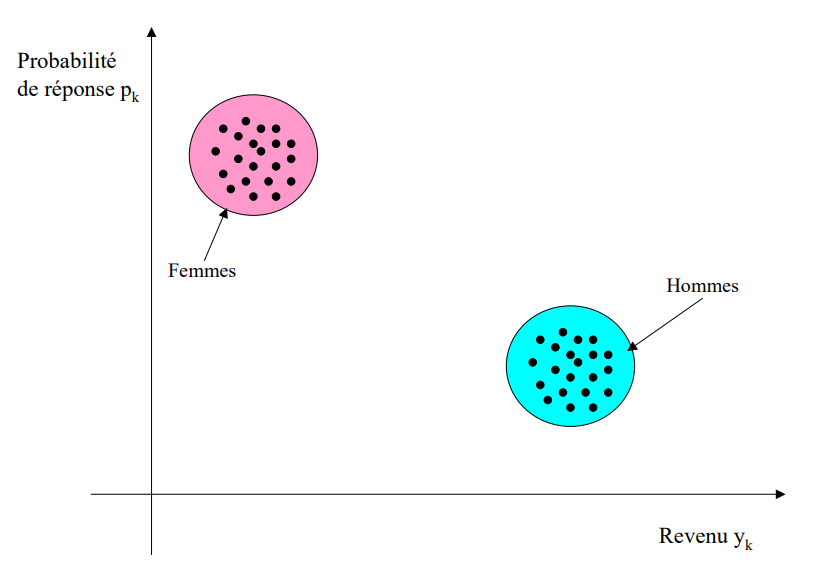
\includegraphics[width=0.9\textwidth]{img/sex.png}
		%	\caption{Legenda da imagem}
		%	\label{fig:label_da_imagem}
	\end{figure}
\end{frame}

\begin{frame}{Exemple}
	Dans une enquête sur le revenu, avec un échantillon initial de 10 000 personnes et un échantillon répondant de taille 8 000, il serait grossier d'estimer $r_k$ par 80\% pour chaque individu. \\ \vspace{0.3cm}
	
	Une solution plus satisfaisante consisterait à considérer les catégories socioprofessionnelles (CSP) si on en dispose pour chaque individu tiré, répondant ou non (ou, mieux, les croisements CSP - âge si l'information existe), et à estimer un taux de réponse
	par catégorie. \\ \vspace{0.3cm}
	
	En effet, il est très probable que les taux de réponse différeront fortement
	selon la catégorie, et on pouffa ainsi obtenir des estimations des $r_k$ plus proches dela réalité. \\ 
	
	
\end{frame}

\begin{frame}{Exemple}
	Par exemple, supposons que l'on obtienne :
	
	\begin{figure}[h]
		\centering
		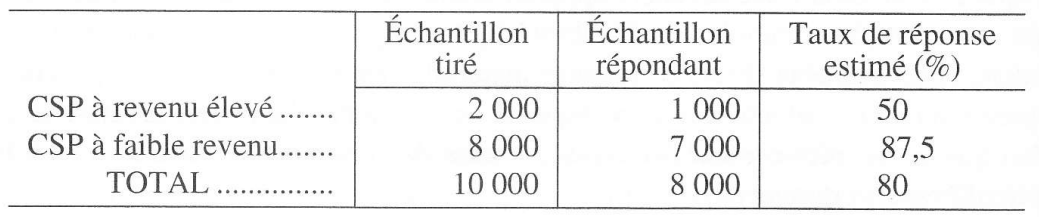
\includegraphics[width=1\textwidth]{img/e.png}
		%	\caption{Legenda da imagem}
		%	\label{fig:label_da_imagem}
	\end{figure}
	
	Ainsi, si $S_{r_1}$ désigne l'échantillon de répondants parmi les CSP à fort revenu (respectivement $S_{r_2}$, parmi les CSP à faible revenu), on utilisera : 
	$$ \hat{T}_r = \sum_{k \in S_{r_1}} \frac{y_k}{\pi_k \times 0.5} + \sum_{k \in S_{r_2}} \frac{y_k}{\pi_k \times 0.875}$$
	
\end{frame}


\begin{frame}{}
	
	\huge \begin{center}
		Le mécanisme de non-réponse ignorable (NMAR)
	\end{center}
	
\end{frame}



\begin{frame}{Mécanisme de non-réponse non ignorable (NMAR)}
Un mécanisme de non-réponse qui n’est pas ignorable est dit non-ignorable (ou Non Missing At Random). \vspace{0.3cm}

\textbf{Cela signifie que la non-réponse dépend de la variable d’intérêt, même une fois que l’on a pris en compte les variables auxiliaires}. \\ \vspace{0.5cm}

Il est très difficile de corriger de la non-réponse non ignorable, ou même de la détecter.\\ \vspace{0.5cm}

\textbf{Exemple :} enquête sur le revenu + non-réponse expliquée par le croisement sexe $\times$ revenu.

\end{frame}



\begin{frame}{Mécanisme de non-réponse ignorable (NMAR)}
	
En pratique, les probabilités de réponse $p_k$ sont inconnues et doivent être estimées. On postule alors un modèle de réponse de la forme 
\[
p_k = f(z_k, \beta_0),
\]
avec 
\begin{itemize}
	\item $z_k$ un vecteur de variables auxiliaires connu sur $S$,
	\item $f(\cdot, \cdot)$ une fonction connue,
	\item $\beta_0$ un paramètre inconnu.
\end{itemize}


\end{frame}

\begin{frame}{Mécanisme de non-réponse ignorable (NMAR)}
	
La liaison en question peut prendre les formes les plus diverses. Une des plus "célèbres" consiste à écrire :\\ 

$$r_k \simeq \frac{a.e^{bX_k}}{1+ a.e^{bX_k}} \Rightarrow Log \frac{r_k}{1+r_k} \simeq Log a + bX_k $$



On parle alors de modèle \textbf{LOGIT} et on sait mettre en œuvre
des procédures pour estimer les paramètres a et b selon certains critères optimaux

\end{frame}

\begin{frame}{Mécanisme de non-réponse ignorable (MAR)}
	
On peut aussi trouver d'autres fonctions de X, qui ont bonne allure et qui
sont toujours comprises entre 0 et 1. Par exemple, on peut s'appuyer sur la fonction de
répartition $\phi(x)$ d'une loi normale centrée réduite, soit


\[ \phi(x) = 
\int_{-\infty}^{x} \frac{1}{\sqrt{2\pi}} e^{-\frac{t^2}{2}} \, dt
\]


et ajuster le modèle $r_k \simeq \phi(a	+ bX_k)$
On parle cette fois de modèle \textbf{PROBIT}, et on sait
également estimer a et b par des techniques appropriées.

\end{frame}

\begin{frame}{}
	\begin{figure}[h]
		\centering
		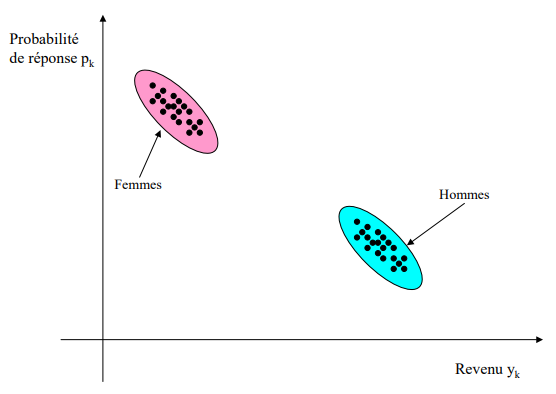
\includegraphics[width=0.9\textwidth]{img/re.png}
		%	\caption{Legenda da imagem}
		%	\label{fig:label_da_imagem}
	\end{figure}
\end{frame}

